\setAuthor{Jaan Kalda}
\setRound{lõppvoor}
\setYear{2024}
\setNumber{G 8}
\setDifficulty{8}
\setTopic{TODO}

\prob{Kolmnurk}
Koondav lääts fookuskaugusega $f$ tekitab täisnurksest kolmnurgast, mille üks nurk on $\SI{30}{\degree}$ kujutiseks kolmnurga, mis on samuti täisnurkne ja mille üks nurk on  $\SI{30}{\degree}$. Kolmnurga hüpotenuus kulgeb piki läätse optilist peatelge. Leidke kolmnurga hüpotenuusi pikkus.


\hint

\solu
\textit{Lahendus 1}:
Esiteks paneme tähele, et õhukeses läätses kujutub sirge sirgeks, kusjuures need sirged lõikuvad läätse tasapinnal. See muutub ilmseks, kui mõtleme neist sirgeist kui valguskiirtest.

Teiseks paneme tähele, et $\SI{30}{\degree}$-ne nurk peab kujutuma  $\SI{60}\degree$-ks nurgaks ja vastupidi. Tõepoolest, kui  $\SI{30}\degree$-ne nurk kujutuks  $\SI{30}\degree$-ks nurgaks ja  $\SI{60}\degree$-ne nurk kujutuks  $\SI{60}\degree$ nurgaks, peaksid esimese tähelepaneku tõttu olema kolmnurk ja tema kujutis peegelsümmeetrilised läätse tasapinna suhtes, mis on vastuolus mitme õhukese läätse omadusega, mh läätse valemiga.

Kolmandaks, optilisel teljel läätsest paremal on vaid üks punkt, kust telje suhtes $\SI{30}\degree$ all lähtuv kiir murdub  $\SI{30}\degree$-se kaldenurgaga kiireks. Tõepoolest, on lihtne näha, et mingist telje punktist $X$, mille kaugus läätsest on suurem fookuskaugusest $f$, $\SI{30}\degree$  all lähtuva kiire kaldenurk peale läätsel murdumist on monotoonne funktsioon punkti $X$ kaugusest fokaaltasandist.

Kolmanda tähelepaneku tõttu on ülesandel vaid üks lahend ning sümmeetria tõttu peavad kolmnurk ja tema kujutis olema täpselt ühesuurused ja samal kaugusel läätsest. Sestap peab algse kolmnurga täisnurk ning kujutiskolmnurga täisnurk olema läätsest võrdsel kaugusel; läätse valemist on lihtne järeldada, et see kaugus on $2f$. Newtoni valem läätse jaoks ütleb, et kui $x_1$ ja $x_2$ on eseme kaugused omapoolsest fokaaltasandist, siis $x_1x_2=f^2$. Olgu täisnurkse kolmnurga täisnurga $C$ projektsioon hüpotenuusile $K$ (vt joonist) ning olgu kolmnurga kõrgus $|CK|=\sqrt 3h$; sellisel juhul kaatetite projektsioonid hüpotenuusile $|AK|=|CK|\tan \SI{30}\degree=h$ ning $|KB|=|CK|\tan \SI{60}\degree=3h$. Sümmeetria tõttu asub $B$ kujutis $B'$ fokaaltasandist sama kaugel, kui nurk $A$, seega Newtoni valem punkti $B$ jaoks omandab kuju $(f-|AK|)(f+|KB|)=(f-h)(f+3h)=f^2$, millest $h=2f/3$ (lahend $h=0$ pole füüsikaline). Nüüd on juba lihtne leida hüpotenuusi pikkuse $|AK|+|KB|=4h=8f/3$.
\begin{center}
  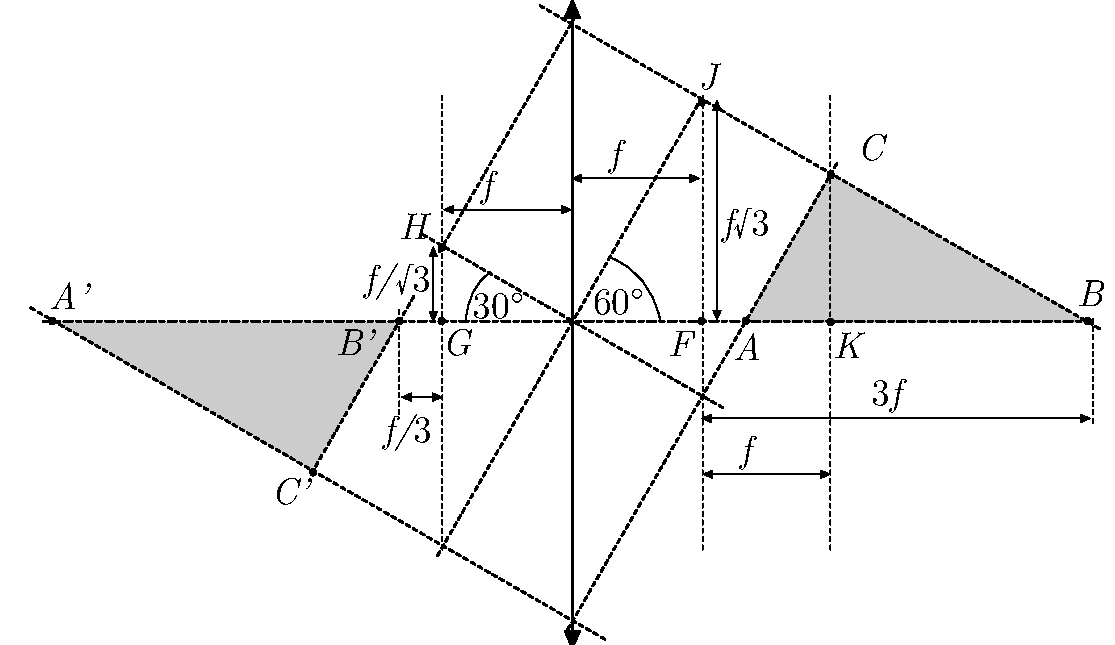
\includegraphics[width=\textwidth]{2024-v3g-08-sol.pdf}
\end{center}

\textit{Lahendus 2}:
Teeme esimesed kaks tähelepanekut nagu 1. lahenduses. Tõmbame läbi läätse keskpunkti kaks sirget, mis kulgevad vastavalt $\SI{30}\degree$ ja $\SI{60}\degree$ nurkade all nii nagu näidatud joonisel. Olgu nende sirgete lõikepunktid fokaaltasanditega vastavalt $J$ ja $H$. On lihtne näha ,et $|JF|=f\tan\SI{60}\degree=\sqrt 3f$ ning $|HG|=f\tan\SI{30}\degree=f/\sqrt 3$. Vasakul pool läätse $\SI{60}\degree$ all kulgevad kiired peavad läbima peale läätsel murdumist punkti $J$, sh peab seda tegema piki kujutiskolmnurga kaatetit $C'B'$ kulgev kiir, mis enne murdumist moodustab optilise teljega $\SI{60}\degree$-se nurga ning pärast läätses murdumist --- $\SI{30}\degree$-se nurga.ning kulgema piki kaatetit $CB$. Täisnurksest kolmnurgast $JFB$ saame avaldada $|FB|=|JF|\tan\SI{60}\degree=3f$ ning täisnurksest kolmnurgast $B'HG$ saame avaldada $|B'G|=|HG|\tan\SI{30}\degree=f/3$. Sümmeetria tõttu $|FA|=|B'G|=f/3$, tänu millele kolmnurga hüpotenuus $|AB|=|FB|-|FA|=3f-f/3=\frac 83f$.
\probend